%%%%%%%%%%%%%%%%%%%%%%%%%%%%%%%%%%%%%%%%%%%%%%%%%%%%%%%%%%%%%%%%%%%%%%
%%                                                                  %%
%%  FINDEC -- manuscript for Digital Finance (Springer Nature)       %%
%%                                                                  %%
%%  Template : Springer Nature sn-jnl.cls v3.1 (December 2024)       %%
%%  Style    : sn-apa  -> APA 7, as Digital Finance requires         %%
%%  Build    : see README.md in this directory                       %%
%%                                                                  %%
%%  Springer Nature requires a SINGLE .tex file at submission.       %%
%%  Do not split this file with \input{...}.                         %%
%%                                                                  %%
%%  Every number in this manuscript traces to an artefact under      %%
%%  eval/results/ or eval/forward/_runs/. See README.md.             %%
%%                                                                  %%
%%%%%%%%%%%%%%%%%%%%%%%%%%%%%%%%%%%%%%%%%%%%%%%%%%%%%%%%%%%%%%%%%%%%%%

\documentclass[pdflatex,sn-apa]{sn-jnl}% APA reference style -- Digital Finance requirement

%%%% Standard packages
\usepackage{graphicx}%
\usepackage{multirow}%
\usepackage{amsmath,amssymb,amsfonts}%
\usepackage{amsthm}%
\usepackage{mathrsfs}%
\usepackage[title]{appendix}%
\usepackage{xcolor}%
\usepackage{textcomp}%
\usepackage{manyfoot}%
\usepackage{booktabs}%
\usepackage{algorithm}%
\usepackage{algorithmicx}%
\usepackage{algpseudocode}%
\usepackage{listings}%

\graphicspath{{figs/}}

\theoremstyle{thmstyleone}%
\newtheorem{theorem}{Theorem}%
\newtheorem{proposition}[theorem]{Proposition}%

\theoremstyle{thmstyletwo}%
\newtheorem{example}{Example}%
\newtheorem{remark}{Remark}%

\theoremstyle{thmstylethree}%
\newtheorem{definition}{Definition}%

\raggedbottom

\begin{document}

\title[Uncertainty and Abstention in Agentic Financial Decision Support]{Uncertainty
and Abstention in Agentic Financial Decision Support: What Should a Financial
Agent Predict?}

%%=============================================================%%
%% NOTE: verify the author block against the journal's own
%% requirements before submission -- in particular ORCIDs, which
%% Digital Finance asks for where available.
%%=============================================================%%

\author*[1]{\sur{Mansi}}\email{mansi.bt22cse@pec.edu.in}

\author[1]{\fnm{Sudesh} \sur{Rani}}\email{sudeshrani@pec.edu.in}

\author[1]{\fnm{Kanu} \sur{Goel}}\email{kanugoel@pec.edu.in}

\affil*[1]{\orgdiv{Department of Computer Science and Engineering},
\orgname{Punjab Engineering College (Deemed to be University)},
\orgaddress{\city{Chandigarh}, \postcode{160012}, \country{India}}}

%%==================================%%
%% Abstract: Digital Finance requires 150--250 words, no undefined
%% abbreviations, no citations, no equations. Current count: ~236.
%%==================================%%

\abstract{Agentic systems for investment decision support almost universally
forecast the direction of price movement, and are almost universally judged on
portfolio return alone. We ask a prior question: given the information such
systems consume, which quantity is worth predicting at all? Measuring five
candidate targets on 196 United States equities over ten years, we find a
pronounced asymmetry. Realised volatility is estimable, with a rank
correlation of $0.554$ against outcome, while return direction is not, at
$-0.074$; a deployed forecaster attains 48.75 percent directional accuracy at
one day, an interval excluding chance from below. We trace the consequence
through FINDEC, an open seven-agent system that plans, gathers evidence,
estimates uncertainty and sizes a position on ordinary processors. Every
exposure rule conditioned on the directional forecast is beaten by a
constant-exposure control holding the system's own average exposure with no
timing, simultaneously on risk-adjusted return, drawdown and return, so
reduced exposure must not be read as risk management. One mechanism survives:
abstaining on low confidence raises accuracy monotonically from 52.1 to 57.5
percent as coverage falls from 100 to 10 percent. We further show that
separating Sharpe ratios differing by 0.30 would require roughly 78 years of
daily data, which bounds what evaluations of this kind can establish, and we
report a sealed prospective test in which an agentic and a numerical
configuration remain statistically indistinguishable.}

\keywords{Agentic artificial intelligence, Financial decision support,
Volatility forecasting, Selective prediction, Backtest evaluation,
Multi-agent systems}

\pacs[JEL Classification]{G11, G14, G17, C53, C58}

\maketitle

%% ==================================================================
\section{Introduction}\label{sec:intro}
%% ==================================================================

Acting on a holding is not one task but six. An investor must understand what
recent news means, extract the relevant facts about the company, analyse the
price history, estimate how uncertain the near future is, judge what downside
is tolerable, and finally decide how much capital the resulting view justifies.
Institutions distribute these among research analysts, quantitative modellers
and risk officers, because they are different problems requiring different
evidence and different competences. Retail investors have none of that division
of labour and must reconcile conflicting sources unaided.

A single prediction model is poorly matched to this structure. It compresses
six heterogeneous questions into one output, usually a direction or a score,
and in doing so discards the intermediate quantities on which a defensible
decision depends. Agentic artificial intelligence offers the natural
alternative: the tasks can be decomposed among specialised agents that
communicate structured evidence rather than opinions, each answerable for the
part of the problem it owns.

Recent systems pursue exactly this decomposition. TradingAgents
\citep{xiao2024tradingagents} assigns analysis, research and execution to
distinct roles, FinRobot \citep{yang2024finrobot} layers language models over
financial tooling, and FinGPT \citep{yang2023fingpt} supplies an open stack for
the same purpose; a recent survey documents how rapidly the area has grown
\citep{fu2025newquant}. Two properties recur across this literature. Evaluation
is almost exclusively end-to-end, reporting a portfolio return, a Sharpe ratio
and occasionally a drawdown. And the quantity predicted is nearly always the
direction of price movement.

Both deserve scrutiny, and the first obstructs the second. An aggregate return
statistic cannot localise a failure, so a system that underperforms offers no
guidance about which component to repair. The most careful long-horizon study
to date finds that language-model investing strategies do not outperform a
passive benchmark across twenty-four years \citep{li2025finsaber}, but because
the evidence is a portfolio aggregate, the mechanism behind the result is not
identified. The question this paper asks is therefore not whether such systems
win, but what is actually happening inside them.

The choice of prediction target is where we begin, because it is rarely
justified. Direction is adopted because it maps conveniently onto a buy or sell
label, not because evidence establishes it as the most estimable quantity
available from the data at hand. If it is not estimable, then every mechanism
conditioned on it, including position sizing, is scaling exposure by noise, and
no amount of architectural sophistication upstream can repair that.

\subsection{Research questions}\label{subsec:rqs}

The paper is organised around one question:

\begin{quote}
How can an agentic financial system combine heterogeneous evidence,
uncertainty estimates and investor risk preferences into decision support that
is more reliable than a direction-only prediction pipeline?
\end{quote}

Four subquestions follow.

\begin{description}
\item[RQ1 (architecture).] Can financial analysis be decomposed into
specialised agents whose outputs remain interpretable and independently
evaluable, rather than only jointly evaluable through portfolio return?

\item[RQ2 (target).] Is estimating uncertainty, volatility and confidence more
useful than attempting to predict raw price direction, and by how much?

\item[RQ3 (selective prediction).] Does permitting the Analyst to abstain on
low-confidence cases improve the reliability of what reaches the agents
downstream?

\item[RQ4 (decision support).] Can a Risk Manager convert those estimates into
risk-sensitive recommendations without mistaking reduced exposure for genuine
predictive skill?
\end{description}

\subsection{Contributions}\label{subsec:contributions}

\begin{itemize}
\item \textbf{A measured predictability asymmetry (RQ2).} Across 196 equities
and ten years, second-moment quantities are substantially more estimable than
direction from an identical information set, and the directional relationship
carries the wrong sign at short horizons.

\item \textbf{Per-agent evaluation (RQ1).} Planner, Analyst and Risk Manager
are scored on metrics appropriate to their own outputs, which localises the
system's failure to the Analyst's target rather than attributing it vaguely to
the architecture.

\item \textbf{Abstention as the surviving mechanism (RQ3).} Confidence-based
withholding raises accuracy monotonically as coverage narrows, with every
interval excluding chance, even though the underlying point forecast is
uninformative.

\item \textbf{The matched-exposure control (RQ4).} Every exposure rule we test
that conditions on the directional forecast is dominated by a constant-exposure
control at the same average exposure. Because reduced exposure lowers drawdown
mechanically, comparison against buy-and-hold alone cannot detect this.

\item \textbf{Sample-size bounds for the literature.} We quantify how much data
a risk-adjusted-return claim requires, and show that holdouts of the length
customary in this field cannot decide the claims routinely made on them.

\item \textbf{A contamination-free prospective test.} A sealed forward test
compares a numerical configuration against a fully agentic one on identical
decisions, at a horizon no model in either arm could have seen in training.
\end{itemize}

We do not claim that FINDEC beats a passive benchmark. It does not, and
Section~\ref{sec:power} shows that at customary sample sizes the question could
not have been settled either way.

%% ==================================================================
\section{Related work}\label{sec:related}
%% ==================================================================

\subsection{Multi-agent financial systems}\label{subsec:related-agents}

Dividing financial analysis among specialised agents improves modularity and
mirrors institutional practice \citep{xiao2024tradingagents,
yang2024finrobot, yang2023fingpt}. These systems demonstrate feasibility but
depend on commercial model endpoints, proprietary data or accelerator hardware,
and each ultimately emits a directional trading decision. FINDEC adopts the
decomposition while keeping the analytical path deterministic and executable on
ordinary processors, which preserves auditability and reproducibility.

\subsection{Evaluation methodology}\label{subsec:related-eval}

\citet{li2025finsaber} constitute the current state of the art in retrospective
evaluation of this class of system: twenty-four years of data, between 63 and
91 symbols per selection strategy, delisted constituents included through
historical index membership, and statistical, reinforcement-learning and
language-model baselines. A passive benchmark attains a Sharpe ratio of $0.703$
against $0.241$ for the strongest agentic competitor, and neither language-model
system produces significant alpha. \citet{nguyen2026reliable} approach the same
problem through taxonomy, arguing for coordination and cost metrics alongside
return.

Two concurrent contributions address look-ahead contamination.
\citet{fonseca2026lookahead} formalise look-ahead freedom as a temporal
non-interference property amenable to verification, and
\citet{benhenda2026lookaheadbench} supply a standardised point-in-time
benchmark, explicitly inviting the instrumentation of further trading agents.
Our contribution is empirical rather than formal: we report what violating the
property was worth inside a real pipeline, and retain a regression suite that
detects it.

The methodological ancestor of this paper is \citet{sullivan1999datasnooping},
who showed that the apparent profitability of technical trading rules largely
evaporates once the search producing them is priced in. The machinery they rely
on remains standard: the reality check of \citet{white2000realitycheck}, the
superior-predictive-ability test of \citet{hansen2005spa}, the
predictive-accuracy comparison of \citet{diebold1995comparing}, and the
stationary bootstrap of \citet{politis1994stationary}. For inference on
differences between correlated Sharpe ratios we use the variance expression of
\citet{jobson1981performance} with the correction of
\citet{memmel2003performance}; \citet{lo2002statistics} and
\citet{bailey2014deflated} give the corresponding standard-error and
multiple-testing treatments.

\subsection{Volatility forecasting}\label{subsec:related-vol}

Unlike returns, volatility exhibits pronounced persistence. The heterogeneous
autoregressive specification of \citet{corsi2009har} regresses future realised
variance on daily, weekly and monthly components and remains a standard
reference point. The conditional-heteroskedasticity model of
\citet{bollerslev1986garch} and the exponentially weighted scheme of
\citet{riskmetrics1996} supply the other conventional baselines, and
\citet{andersen1998answering} established that such models forecast accurately
once the target is measured with realised rather than squared daily returns.
\citet{patton2011volatility} showed that when the target is observed only
through a noisy proxy many loss functions rank forecasts incorrectly, and
identified squared error and QLIKE as robust choices; we adopt QLIKE as primary
for that reason.

Whether a volatility estimate translates into performance is separate.
\citet{moreira2017volatility} report that scaling exposure inversely with
recent volatility improves risk-adjusted returns at the level of the market
portfolio, a finding our single-name results do not reproduce; we return to the
discrepancy in Section~\ref{subsec:disc-uncertainty}.

\subsection{Selective prediction}\label{subsec:related-selective}

Allowing a predictor to decline is an old idea, formalised by
\citet{chow1970optimum} as a trade-off between error and rejection rate and
developed for the modern setting by \citet{elyaniv2010foundations} and
\citet{geifman2017selective}. Its application to financial agents is direct but
largely unexploited: an agent whose point forecast is uninformative may
nonetheless rank its own reliability, and the accuracy attainable on the subset
it retains is the quantity of interest.

\subsection{Classical baselines}\label{subsec:related-baselines}

Any claim of a contribution from an agentic architecture must clear the
classical rules it may be reproducing. \citet{brock1992simple} document
moving-average rules and \citet{moskowitz2012timeseries} establish time-series
momentum; both are implemented as baselines here. The efficiency argument of
\citet{fama1970efficient} supplies the null against which our directional
results are read.

%% ==================================================================
\section{The FINDEC architecture}\label{sec:arch}
%% ==================================================================

FINDEC is an open system organised as seven cooperating agents behind a web
application and a service tier. The whole analytical path executes on ordinary
processors with no accelerator hardware, which matters here only because it
makes the evaluation cheap to reproduce, not because it is itself a
contribution. Figure~\ref{fig:arch} shows the arrangement and the contract
carried on every edge.

\subsection{The two planes}\label{subsec:planes}

The agents divide into two planes, and the division is the system's load-bearing
architectural commitment rather than a taxonomy imposed after the fact.

The \emph{control plane} decides what work to do. It comprises the Planner,
which turns a query into a task graph, and the Optimizer, which judges whether
the returned evidence supports a decision and re-queries when it does not. Both
are language-model driven.

The \emph{decision plane} decides what the market will do. It comprises the
Researcher, Market, Analyst, Fundamentals and Risk Manager agents. Every one is
numerical and deterministic given its inputs, and no language model appears
anywhere in it.

The separation is not stylistic. Current language models were trained on text
covering any historical window a retrospective evaluation might use, so a model
placed in the decision path is recalling the period rather than forecasting it,
and every backtest number computed through it becomes uninterpretable. This is
the contamination \citet{li2025finsaber} identify as unaddressed in their own
study. Confining the language model to the control plane leaves the decision
plane backtestable without contamination, which is what permits
Sections~\ref{subsec:eval-direction} through \ref{subsec:eval-voltarget} to be
read as measurements at all. The cost is that the control plane cannot itself be
backtested, and we do not attempt to; it is evaluated prospectively in
Section~\ref{subsec:eval-forward} and by component in
Section~\ref{subsec:eval-components}.

A second consequence is economic. Because the Optimizer runs a deterministic
conflict screen before consulting a model at all, most queries complete with no
language-model call whatever, which is visible in the prospective test as a mean
of 0.20 calls per agentic decision.

\begin{figure}[h]
\centering
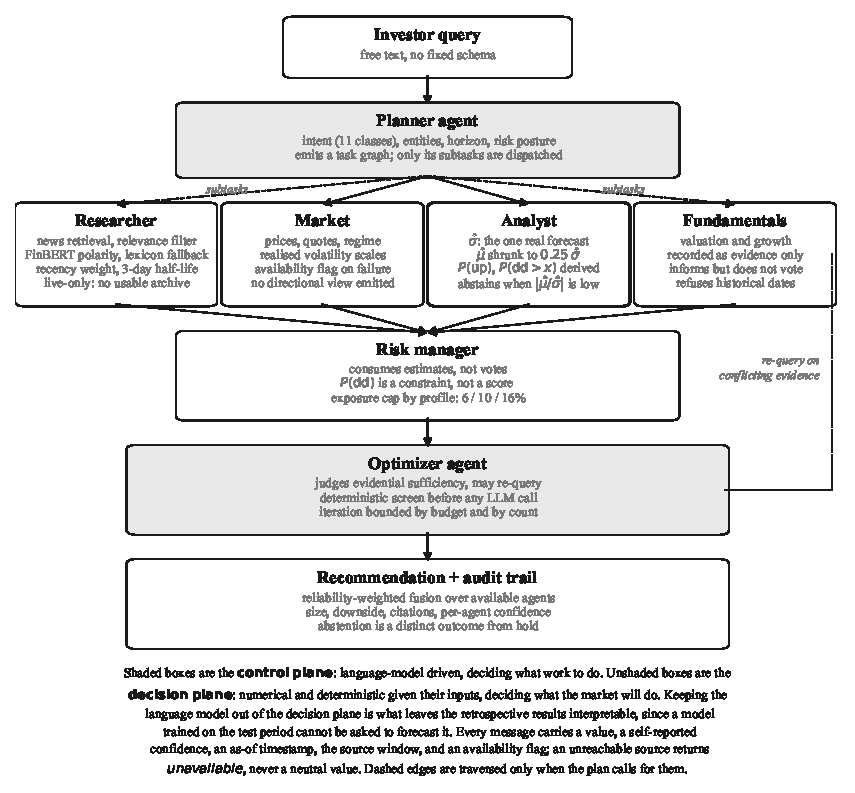
\includegraphics[width=\textwidth]{fig_architecture}
\caption{FINDEC's seven agents and the contract between them. Shaded boxes are
the control plane, which is language-model driven and decides what work to do;
unshaded boxes are the decision plane, which is numerical and deterministic and
decides what the market will do. The Planner decides which agents run, so dashed
edges are traversed only when the plan calls for them, and the Optimizer may
re-query the decision plane when the returned evidence conflicts. The Analyst,
drawn with a heavier border as the component this paper examines most closely,
emits a distribution and a calibrated confidence rather than a directional
label; the Risk Manager consumes those estimates as constraints rather than as
votes.}\label{fig:arch}
\end{figure}

\subsection{What makes this agentic rather than a pipeline}\label{subsec:agentic}

The distinction matters, because a decomposition into three modules called
sequentially is not an agentic system and should not be described as one. Seven
properties separate them here, and each is observable in the execution trace
rather than asserted in prose.

\emph{Task decomposition.} The Planner converts free text into a structured
task graph naming intent, entities, decision horizon and required subtasks. The
graph is data, not control flow.

\emph{Dynamic routing.} The orchestrator dispatches exactly the subtasks the
graph names and no others, honouring declared dependencies in waves. A
definitional query dispatches nothing at all; the agent set is a function of the
query, not a constant. The prospective test of
Section~\ref{subsec:eval-forward} shows this concretely: on identical inputs the
numerical configuration invoked one agent per decision while the agentic
configuration invoked four of the five decision-plane agents available to it,
the Fundamentals agent being omitted by the plan rather than by configuration.

\emph{Specialised roles with distinct evidence.} The Researcher consumes text,
the Market agent consumes prices, the Analyst consumes engineered features and
the Risk Manager consumes only other agents' outputs. No two agents see the
same input, which is what makes per-agent evaluation meaningful under RQ1.

\emph{Structured inter-agent communication.} Every message is typed and carries
a value, the agent's self-reported confidence, the timestamp of the newest datum
consulted, the window it was drawn from, and an availability flag. A decision
can therefore be reconstructed exactly, and any information postdating it
detected. This is the practical form of the non-interference property that
\citet{fonseca2026lookahead} formalise.

\emph{Explicit failure handling.} An agent unable to reach its source returns
\emph{unavailable}, never a neutral value. Synthesis then reweights over the
agents that did respond. The distinction is not cosmetic: an earlier revision
treated missing sentiment as neutral sentiment, which anchored the aggregate
score at its midpoint and suppressed action entirely.

\emph{Confidence propagation.} Confidence travels with the estimate and is
consumed downstream as a quantity, not discarded at the module boundary. Because
the Analyst's confidence is calibrated against realised outcomes
(Section~\ref{subsec:eval-calibration}), a stated value corresponds to an
observed frequency.

\emph{Risk-conditioned decision making.} The Risk Manager treats an estimated
downside probability as a constraint on exposure rather than as another additive
score, so a sufficiently adverse estimate can veto a recommendation that every
other signal supports.

Two post-conditions are enforced after planning rather than requested of the
model, since a prompt expresses an intention while a post-condition enforces
one. Definitional queries dispatch no agents. Queries placing the user's capital
at risk always attach a downside estimate, whether or not downside was asked
about.

%% ==================================================================
\section{Agent design}\label{sec:agents}
%% ==================================================================

\subsection{Planner agent}\label{subsec:planner}

The Planner classifies a query into one of eleven intents and emits a
schema-validated task graph. The vocabulary derives from observed usage rather
than invention: published analysis of retail questions put to a financial
assistant finds that interpretation and screening dominate while explicit
requests for advice are a small minority. The Planner resolves company names to
exchange symbols, relative horizons to day counts, and infers risk posture from
how loss tolerance is described rather than from an explicit label alone.

\subsection{Researcher agent}\label{subsec:researcher}

The Researcher assembles structured evidence rather than prose. Retrieved
articles are filtered for financial relevance, deduplicated by source, and
scored by a domain-adapted encoder \citep{araci2019finbert} with a lexicon
scorer retained as fallback. Each article carries a recency weight with a
three-day half-life, and the agent returns an aggregate polarity, an
agreement-based confidence and the citations backing them.

Its scope requires a statement. Historical news at the access tier used here
extends roughly thirty days into the past, so the Researcher cannot participate
in a decade-long retrospective evaluation. Even with an archive, scoring
historical headlines with a pretrained encoder would introduce a subtler
difficulty, since the encoder's parameters may already encode the period under
test; this is the contamination \citet{li2025finsaber} name as an unaddressed
limitation of their own study. The Researcher is therefore evaluated only
prospectively and is excluded from the retrospective results of
Section~\ref{sec:results}.

\subsection{Analyst agent}\label{subsec:analyst}

The Analyst is the research object of this paper, because everything downstream
conditions on what it produces.

\subsubsection{Why the original design was abandoned}\label{subsubsec:wrong-target}

The original Analyst emitted a directional label from an ensemble of ridge
regression and logistic classification over engineered features. Evaluated at
scale rather than on a handful of names, the rank correlation between predicted
and realised direction proved negative at every horizon tested
(Section~\ref{subsec:eval-direction}). A point estimate of an unforecastable
quantity is not a useful object, and any mechanism that scales exposure by such
an estimate scales it by noise.

\subsubsection{Feature construction}\label{subsubsec:features}

Features are computed from a strictly backward-looking window. Beyond
conventional technical terms, the set emphasises dispersion rather than
direction: realised volatility over multiple scales, the ratio between short-
and long-horizon volatility, downside semivariance, rolling skewness and
kurtosis, drawdown depth and time since peak, volume relative to its own trend,
and return relative to a market proxy. All are standardised using statistics
drawn from the training window alone.

\subsubsection{Estimating a distribution rather than a label}\label{subsubsec:distribution}

The redesigned Analyst emits a distribution. Its governing principle follows
from the measured asymmetry: estimate the second moment, remain honest about
the first, and derive the remainder. For horizon $h$, dispersion is estimated
from realised variance while the central estimate is shrunk toward zero and
capped at a small fraction of the estimated standard deviation,
\begin{equation}\label{eq:dist}
\hat{\sigma}_h = \sqrt{h}\,\hat{\sigma}_{\text{daily}},
\qquad
|\hat{\mu}_h| \leq \kappa\,\hat{\sigma}_h,
\end{equation}
with $\kappa = 0.25$. The asymmetry is deliberate. Asserting a mean produced a
negative information coefficient; estimating dispersion honestly leaves the
output useful regardless, because sizing keys on the ratio
$\hat{\mu}_h/\hat{\sigma}_h$ rather than on the level of either term.

Given $\hat{\sigma}_h$, further quantities follow analytically rather than from
separately fitted models. The probability of appreciation is
$\Phi(\hat{\mu}_h/\hat{\sigma}_h)$, with $\Phi$ the standard normal
distribution function. The probability that the path falls a fraction $x$ below
its starting value within the horizon follows from the reflection principle,
\begin{equation}\label{eq:dd}
P(\text{drawdown} > x) = 2\,\Phi\!\left(\frac{-x}{\hat{\sigma}_h}\right),
\end{equation}
and expected maximum drawdown scales with $\hat{\sigma}_h$. Deriving these
rather than fitting them separately guarantees mutual consistency, since
$P(\text{up})$, the information ratio and expected drawdown cannot contradict
one another, and it concentrates estimation risk in one place where it can be
measured. Section~\ref{subsec:eval-calibration} measures it, and finds it
wanting.

An earlier revision instead simulated paths under geometric Brownian motion
whenever the fitted model was unavailable. That fallback was removed: it
produced outputs formally indistinguishable from fitted ones while carrying no
information about the security in question, and no downstream consumer could
tell the difference.

\subsubsection{The full output contract}\label{subsubsec:contract}

The Analyst emits expected return, expected volatility, probability of an
upward move, calibrated confidence, cross-sectional percentile rank, a regime
label, a downside probability, and an abstention decision. This is a
substantially richer object than a directional label, and it is what permits
the Risk Manager to size a position without needing to know which way the price
will move. Because ranking a security against its peers is a different problem
from forecasting its absolute movement, the percentile rank is computed across
the day's universe and cannot be produced by per-ticker invocation.

\subsubsection{Confidence and abstention}\label{subsubsec:abstention}

A raw confidence is formed from $|\hat{\mu}_h/\hat{\sigma}_h|$ and mapped
through a reliability curve fitted on realised outcomes, so a stated value
corresponds to an observed frequency rather than to model self-report. When the
ratio falls below a threshold the Analyst abstains, returning no view rather
than a weak one. Abstention is a first-class output: given the evidence of
Section~\ref{subsec:eval-abstention}, no view is frequently the correct answer,
and a system unable to express it will manufacture one.

\subsection{Risk Manager agent}\label{subsec:riskmgr}

The Risk Manager consumes estimates, not votes. Position scale follows from the
volatility estimate against a risk budget; the drawdown probability of
Equation~\eqref{eq:dd} acts as a constraint rather than a score, capping
exposure when it exceeds the profile's tolerance; and calibrated confidence
modulates size within that budget. An abstaining Analyst suppresses the
recommendation entirely, which the interface distinguishes from a hold.
Profiles cap exposure at 6, 10 and 16 percent of capital.

Position changes take effect on the session after the one whose closing data
produced them. Applying a decision to the same session's return would let
information in that closing price influence a position notionally taken
beforehand; Section~\ref{subsec:disc-eval} reports what that error was worth
when it was present.

\subsection{Fundamentals agent}\label{subsec:fundamentals}

The Fundamentals agent retrieves valuation and growth measures and records them
as evidence supporting the written explanation. It casts no directional vote.
The one field that would supply one is a broker consensus rating, and routing
that into the fusion would amount to reporting other analysts' forecasts as the
system's own, so it is recorded and excluded from the vote.

The agent refuses historical dates by design. Its source returns whatever the
fundamentals are at the time of the call, with no point-in-time parameter, so
serving a current price-to-earnings ratio for a decision dated months earlier
would be textbook look-ahead, and invisible downstream because the number looks
entirely ordinary. When the requested as-of date is more than a couple of days
old the agent returns \emph{unavailable} and says why. This is the availability
mechanism of Section~\ref{subsec:agentic} used deliberately as a leakage
control, and it is the reason the agent contributes nothing to the retrospective
results of Section~\ref{sec:results}.

\subsection{Optimizer agent}\label{subsec:optimizer}

The Optimizer sits between the router and the fusion step. Given the agents'
results it judges whether they collectively support a decision and, when they do
not, which agent should be asked what instead. It is the second of the two
control-plane agents and the only one that can cause work to be repeated.

Two properties keep it tractable. It produces no numbers: numeric synthesis
belongs to the fusion weighting, which is a function of measurable state and is
therefore auditable, whereas a language model asked to emit a weight would put
an unauditable term into every downstream figure. And a deterministic conflict
screen runs before any model call, so the model is consulted only when the
screen finds a genuine disagreement. Iteration is bounded twice over, by an
explicit iteration count and by the model-call budget, because an agent loop
permitted to decide its own stopping condition is an agent loop that can fail
to stop.

%% ==================================================================
\section{Experimental protocol}\label{sec:protocol}
%% ==================================================================

\subsection{Data and splits}\label{subsec:protocol-data}

Retrospective results use daily data for 196 United States equities spanning
ten years, with at least two constituents per sector. Models refit on a
trailing window and are scored only on subsequent unseen observations, so every
reported statistic is walk-forward and out of sample. Parameters were selected
on a tuning segment and the holdout segment was scored once.

\subsection{Leakage controls}\label{subsec:protocol-leakage}

Three controls apply throughout. Features are computed from strictly
backward-looking windows and standardised with training-window statistics only.
Position changes are lagged by one session, as described in
Section~\ref{subsec:riskmgr}. And nine regression tests assert temporal
alignment directly, comparing each decision's timestamp against the timestamps
of the data that produced it. The tests exist because the defect they detect
was present: Section~\ref{subsec:disc-eval} reports its magnitude.

\subsection{Costs and cash}\label{subsec:protocol-costs}

The execution-policy experiment of Section~\ref{subsec:eval-voltarget} charges
5 basis points of turnover on each rebalance and credits idle capital at a
4 percent annual rate. The component ablation of
Section~\ref{subsec:eval-sizing} credits idle capital at the same rate but does
not charge turnover; since the arms it compares differ in exposure rather than
in trading frequency, and since the matched-exposure control trades strictly
less than the policy it beats, charging turnover would widen the gap we report
rather than narrow it.

\subsection{Statistical procedures}\label{subsec:protocol-stats}

Accuracy figures carry 95 percent Wilson intervals
\citep{wilson1927probable}, which behave correctly near the boundary and at the
small subsample sizes arising under abstention. Sharpe-ratio differences are
tested with a stationary bootstrap \citep{politis1994stationary} to respect
serial dependence, and the choice among risk profiles is priced with the
superior-predictive-ability test of \citet{hansen2005spa}. Where a forecast is
compared at overlapping horizons we also report the non-overlapping subsample,
since overlapping windows inflate effective sample size. Volatility forecasts
are ranked by QLIKE, which remains valid under a noisy proxy
\citep{patton2011volatility}, with mean squared error, rank correlation and
Mincer--Zarnowitz regressions reported alongside.

\subsection{The prospective arm}\label{subsec:protocol-forward}

Because any pretrained component may have encountered the retrospective period
during training, we additionally run a sealed forward test. Predictions are
committed with a cryptographic seal and an as-of date before the outcome
exists, and scored only after the horizon elapses. Two configurations run in
parallel on identical inputs: a numerical arm invoking the Analyst alone, and a
fully agentic arm running the complete control plane, whose plans dispatched
four of the five decision-plane agents. This is the only experiment in the paper
that is contamination-free by construction, and the only one in which the
control plane participates at all.

\subsection{Known biases}\label{subsec:protocol-bias}

The universe was selected at the end of the sample, so every constituent
survived the period. This survivorship flatters all reported columns and
applies equally to the system and to its baselines. It is the one bias
\citet{li2025finsaber} handle properly and we do not.

%% ==================================================================
\section{Results}\label{sec:results}
%% ==================================================================

Table~\ref{tab:agents} summarises each agent against a metric appropriate to
its own output. Reporting them separately is what answers RQ1: it localises the
system's failure to the Analyst's choice of target rather than attributing it
to the architecture.

\begin{table}[h]
\caption{Per-agent evaluation. Each agent is scored on its own output rather
than through a portfolio aggregate. Baselines are the value the metric takes
under no skill, except for the Planner, where it is a published supervised
classifier, and the Risk Manager, where it is the matched-exposure
control.}\label{tab:agents}%
\begin{tabular*}{\textwidth}{@{\extracolsep\fill}lllcc@{}}
\toprule
Agent & Metric & Sample & Result & Baseline \\
\midrule
Planner      & Intent accuracy                & 33 queries    & 0.727    & 0.75 \\
Researcher   & Retrospective coverage         & ---           & n/a      & --- \\
Analyst      & Rank corr., direction          & 43{,}512 obs. & $-0.074$ & 0 \\
Analyst      & Rank corr., volatility         & 43{,}512 obs. & $+0.554$ & 0 \\
Analyst      & Directional accuracy, $h{=}1$  & 8{,}814 dec.  & 0.4875   & 0.50 \\
Analyst      & Accuracy at 10\% coverage      & 570 dec.      & 0.5754   & 0.50 \\
Risk Manager & Sharpe vs.\ matched exposure   & 10 names, 10 yr & 0.381  & 0.539 \\
\botrule
\end{tabular*}
\footnotetext{The Researcher is not scored retrospectively for the reason given
in Section~\ref{subsec:researcher}; it appears in the prospective test of
Section~\ref{subsec:eval-forward}.}
\end{table}

\subsection{Experiment A: is direction predictable?}\label{subsec:eval-direction}

Table~\ref{tab:analyst} reports, for each candidate target, the rank
correlation between a forecast built from trailing information and the realised
outcome, together with the deployed Analyst's directional performance at three
horizons. Panel (a) of Figure~\ref{fig:results} plots the asymmetry.

\begin{table}[h]
\caption{Predictability of candidate targets, and deployed directional
performance. Upper block: 43,512 out-of-sample observations across 196 equities
at a 21-day horizon. Lower block: 8,814 decisions across 39 equities, with 95
percent Wilson intervals, the Spearman information coefficient, and a binomial
$p$-value against chance.}\label{tab:analyst}%
\begin{tabular*}{\textwidth}{@{\extracolsep\fill}lcc@{}}
\toprule
Target & Rank correlation & $R^2$ \\
\midrule
Direction of return          & $-0.0744$ & 0.014 \\
Magnitude of return          & $+0.2489$ & 0.108 \\
Realised volatility          & $+0.5543$ & 0.286 \\
Forward maximum drawdown     & $-0.3199$ & 0.084 \\
\midrule
Horizon & Accuracy [95\% CI] & IC \quad ($p$) \\
\midrule
1 day    & 0.4875 \enskip [0.4771, 0.4980] & $-0.0257$ \enskip (0.020) \\
5 days   & 0.5021 \enskip [0.4916, 0.5126] & $-0.0195$ \enskip (0.701) \\
21 days  & 0.5073 \enskip [0.4968, 0.5178] & $-0.0128$ \enskip (0.174) \\
21 days, non-overlapping & 0.4944 \enskip [0.4763, 0.5125] & $-0.0464$ \enskip (0.554) \\
\botrule
\end{tabular*}
\footnotetext{The two negative rank correlations carry opposite meanings. For
direction the forecast is anti-predictive. For drawdown the negative sign is
the expected relationship, since higher trailing volatility predicts a deeper
subsequent fall.}
\end{table}

Volatility is roughly seven times more predictable than direction, and the
directional relationship carries the wrong sign. At one day the accuracy
interval lies wholly below $0.50$ and the binomial test rejects chance at
$p=0.020$: the forecast is significantly worse than chance, not merely
uninformative. At longer horizons it is indistinguishable from chance, and the
21-day result does not survive restriction to non-overlapping windows, where
accuracy falls to $0.4944$. Only 13 of 39 names exceed $0.50$ at one day.

The cross-sectional information coefficient tells the same story: averaged over
95 rebalance dates the mean rank IC is $+0.016$ with an information ratio of
$0.067$ ($t=0.65$, $p=0.52$), statistically indistinguishable from zero. Read
against \citet{fama1970efficient}, the short-horizon result is not evidence of
exploitable reversal so much as evidence that whatever signal the features
carry is weaker than the noise the estimator introduces. The answer to the
first half of RQ2 is therefore negative, and it is negative decisively.

\begin{figure}[h]
\centering
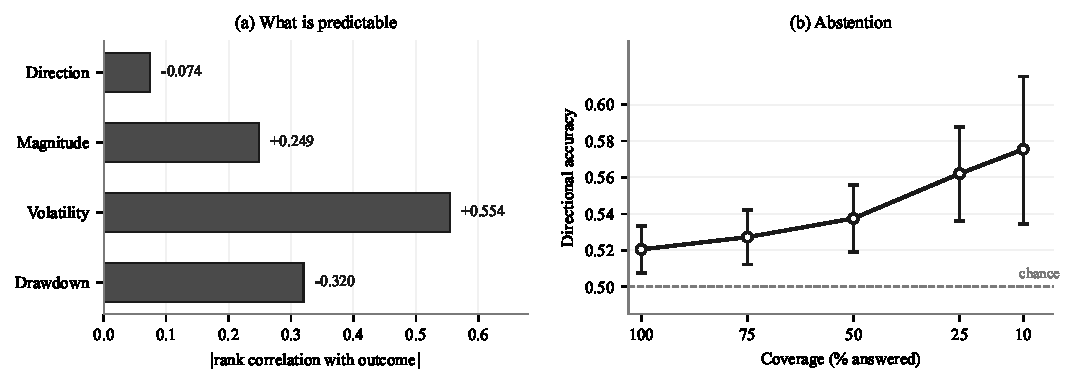
\includegraphics[width=\textwidth]{results_panels}
\caption{The two central results. (a) Strength of the relationship between a
forecast built from trailing information and the realised outcome, over 43,512
out-of-sample observations at a 21-day horizon; bar length is the magnitude of
the rank correlation and the signed value is annotated. (b) Directional
accuracy against coverage under confidence-based abstention, with 95 percent
Wilson intervals; the dashed line marks chance.}\label{fig:results}
\end{figure}

\subsection{Experiment B: is volatility predictable?}\label{subsec:eval-vol}

Table~\ref{tab:vol} and Figure~\ref{fig:vol} compare four volatility models on
four metrics, in two independent evaluation runs.

\begin{table}[h]
\caption{Volatility forecast comparison at a 21-day horizon. QLIKE is the
primary metric and lower is better; MSE is on variance units. IC is the rank
correlation with realised volatility and MZ denotes the Mincer--Zarnowitz
regression of realised on forecast, whose slope is 1 under unbiasedness. The
final column is a second, independent run on a different sample, reported
because it reverses the ranking.}\label{tab:vol}%
\begin{tabular*}{\textwidth}{@{\extracolsep\fill}lrrrrr@{}}
\toprule
& \multicolumn{4}{@{}c@{}}{Universe run ($n=1{,}900$, 20 names)} & Redesign run \\
\cmidrule{2-5}
Model & QLIKE & MSE ($\times 10^{-7}$) & IC & MZ slope & QLIKE ($n=5{,}700$) \\
\midrule
Random walk            & $-6.595$ & 4.486 & 0.609 & 0.461 & $-6.724$ \\
Unconditional mean     & $-6.746$ & 3.643 & 0.575 & 0.872 & --- \\
EWMA ($\lambda{=}0.94$)& $-6.737$ & 3.904 & 0.635 & 0.536 & $-6.823$ \\
HAR-RV                 & $-6.711$ & 3.593 & 0.655 & 1.138 & $-6.789$ \\
\botrule
\end{tabular*}
\end{table}

\begin{figure}[h]
\centering
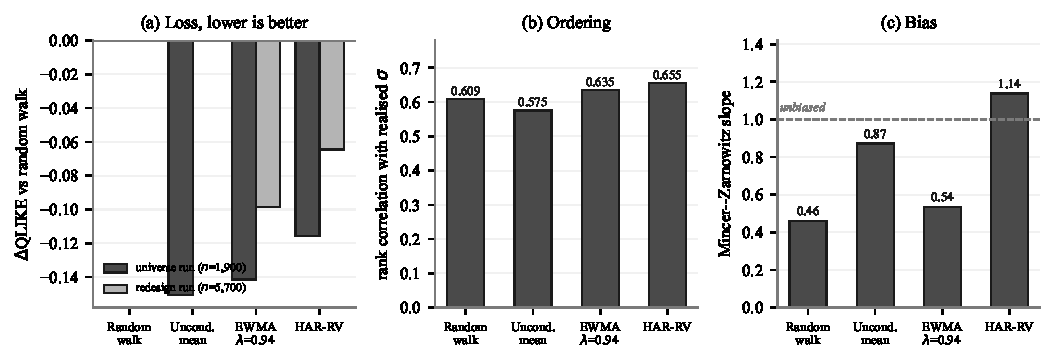
\includegraphics[width=\textwidth]{fig_volatility}
\caption{Four volatility models on three criteria. (a) QLIKE relative to the
random walk in both runs; every conditional model improves on the random walk,
but the two runs disagree about which improves most. (b) Rank correlation with
realised volatility, where HAR-RV leads. (c) Mincer--Zarnowitz slope, where
HAR-RV is closest to unbiased and the exponentially weighted estimator is the
most attenuated.}\label{fig:vol}
\end{figure}

Volatility is emphatically estimable: rank correlations between $0.58$ and
$0.66$ against a directional figure of $-0.07$ from the same information set.
That is the finding RQ2 turns on, and it is robust across both runs and every
model considered.

The ranking among models is not. In the universe run the best QLIKE belongs to
the \emph{unconditional mean}, which uses no conditioning information at all;
in the redesign run the exponentially weighted estimator is best and HAR-RV
beats the random walk but not EWMA. We report this rather than selecting the
run in which the sophisticated model wins. Two observations reconcile it. QLIKE
penalises errors in the level of variance, and the unconditional mean is
well-centred by construction even though it cannot order anything, which is
visible in its rank correlation of $0.575$, the lowest of the four. HAR-RV,
conversely, wins the two criteria a sizing rule actually needs: it ranks best
($\text{IC}=0.655$) and is nearest to conditionally unbiased ($\text{MZ slope}
= 1.138$ against $0.536$ for EWMA and $0.461$ for the random walk).

The practical conclusion is that model choice should follow the use. A rule
that scales exposure by relative volatility needs ordering and conditional
unbiasedness, which favours HAR-RV; a rule that needs a calibrated level is
barely served better by any of them than by a constant. Reporting only QLIKE,
as is common, would have selected the unconditional mean and concealed this.

\subsection{Experiment C: are the derived risk quantities calibrated?}\label{subsec:eval-calibration}

Because Equation~\eqref{eq:dd} derives downside probabilities from
$\hat{\sigma}_h$ rather than fitting them, all the estimation risk is
concentrated in one place. Table~\ref{tab:calib} and Figure~\ref{fig:calib}
measure it at three drawdown thresholds.

\begin{table}[h]
\caption{Calibration of derived downside probabilities, HAR-RV volatility
model, 21-day horizon, 3,800 forecasts. ECE is the expected calibration error.
The base rate is the unconditional frequency of the event.}\label{tab:calib}%
\begin{tabular*}{\textwidth}{@{\extracolsep\fill}lrrrrrl@{}}
\toprule
Threshold & Mean predicted & Realised & Brier & Base-rate Brier & ECE & Verdict \\
\midrule
$x=5\%$  & 0.4016 & 0.3882 & 0.2377 & 0.2375 & 0.0636 & loses \\
$x=10\%$ & 0.1339 & 0.1547 & 0.1301 & 0.1308 & 0.0500 & beats \\
$x=20\%$ & 0.0140 & 0.0245 & 0.0245 & 0.0239 & 0.0168 & loses \\
\botrule
\end{tabular*}
\footnotetext{Across the pooled reliability curve: worst-bin gap $0.265$, curve
slope $-0.064$ per bin, and mean bias in $\hat{\sigma}$ of $-11.0$ percent.}
\end{table}

\begin{figure}[h]
\centering
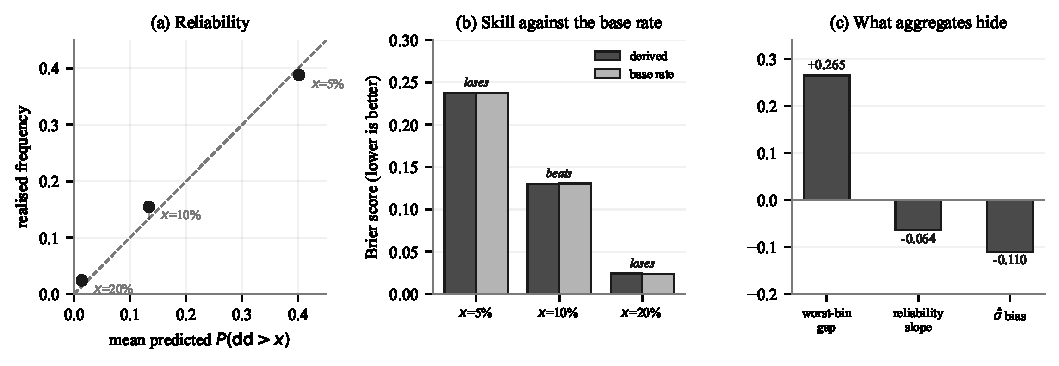
\includegraphics[width=\textwidth]{fig_calibration}
\caption{Calibration of the derived downside probabilities. (a) Mean predicted
probability against realised frequency at three thresholds; the model overstates
risk at the common threshold and understates it at the rare one. (b) Brier
score against the corresponding base rate, which the derived probability beats
at only one of three thresholds. (c) The diagnostics an aggregate score
conceals: a worst-bin gap of $0.265$, a reliability curve sloping the wrong
way, and an $11$ percent underestimate of
volatility.}\label{fig:calib}
\end{figure}

Three findings. First, the derived probabilities beat their own base rate at
only one of three thresholds, and the margin there is slight ($0.1301$ against
$0.1308$). A risk quantity that barely improves on the unconditional frequency
is not yet doing work.

Second, and more instructive, the aggregate can look acceptable while the
reliability curve is structurally wrong. The pooled expected calibration error
of $0.050$ at $x=10\%$ is unremarkable, but the reliability curve slopes at
$-0.064$ per bin with a worst-bin gap of $0.265$. The slope is the diagnostic
that matters: the model overstates risk precisely where it predicts risk to be
highest, which is the direction of error least useful to a constraint that is
supposed to bind in dangerous states. Reporting only a pooled Brier or ECE
would have hidden this entirely.

Third, $\hat{\sigma}$ is biased low by $11.0$ percent on average. Since every
derived quantity in Section~\ref{subsubsec:distribution} is a monotone function
of $\hat{\sigma}$, a systematic underestimate of dispersion propagates to
systematically understated downside. Concentrating estimation risk in one place
made this measurable in a single number; it did not make it small.

\subsection{Experiment D: does abstention help?}\label{subsec:eval-abstention}

Table~\ref{tab:abstain} and panel (b) of Figure~\ref{fig:results} report
accuracy as a function of coverage, where coverage is the proportion of queries
on which the system commits to a view and abstention removes the least
confident.

\begin{table}[h]
\caption{Accuracy against coverage under confidence-based abstention. 5,700
out-of-sample decisions with 95 percent Wilson bounds.}\label{tab:abstain}%
\begin{tabular*}{\textwidth}{@{\extracolsep\fill}rrcc@{}}
\toprule
Coverage & $n$ & Accuracy & 95\% CI \\
\midrule
100\% & 5{,}700 & 0.5205 & [0.5075, 0.5335] \\
75\%  & 4{,}275 & 0.5273 & [0.5123, 0.5422] \\
50\%  & 2{,}850 & 0.5375 & [0.5192, 0.5558] \\
25\%  & 1{,}425 & 0.5621 & [0.5362, 0.5877] \\
10\%  &   570   & 0.5754 & [0.5345, 0.6154] \\
\botrule
\end{tabular*}
\end{table}

Accuracy rises monotonically as the system answers less often, from $52.1$ to
$57.5$ percent, and every interval excludes chance. This is the paper's
strongest result and the answer to RQ3. The Analyst cannot forecast direction,
yet its confidence ranks its own reliability: the ordering carries information
the point estimate does not. It is the risk--coverage trade-off of
\citet{chow1970optimum} recovered in a financial setting.

The mechanism also fits the agentic framing. An agent that emits a calibrated
estimate together with an explicit abstention can be audited against observed
frequency; an agent that emits a buy or sell label carries no claim that can be
checked. Withholding is therefore not a degradation of the interface but a
precondition for evaluating it.

We report one qualification in Section~\ref{subsec:eval-forward}: this
monotonicity does not yet replicate in the prospective sample, which is far too
small to resolve it.

\subsection{Experiment E: does the sizing policy add skill?}\label{subsec:eval-sizing}

Conditioning exposure on an uninformative forecast carries a measurable cost.
We compare the sized policy against a control that holds the system's own
average exposure every day with no timing whatsoever. The control separates
genuine risk management from simply holding less, and it is the instrument RQ4
requires.

\begin{table}[h]
\caption{Exposure ablation with a matched-exposure control. Ten equities, ten
years, high-risk profile. Avg.\ exp.\ is the mean fraction of capital
invested.}\label{tab:ablation}%
\begin{tabular*}{\textwidth}{@{\extracolsep\fill}lrrrr@{}}
\toprule
Arm & Avg.\ exp. & Sharpe & Ann.\ return (\%) & Max.\ drawdown (\%) \\
\midrule
Full system                     & 0.42 & 0.381 &  9.97 & $-38.0$ \\
No position sizing              & 0.53 & 0.361 & 10.30 & $-51.7$ \\
No confidence (fixed 10\%)      & 0.05 & 0.361 &  4.96 & $-3.8$  \\
No volatility targeting         & 0.44 & 0.387 & 10.65 & $-51.7$ \\
Always invested (harness check) & 1.00 & 0.497 & 16.52 & $-71.7$ \\
Buy and hold                    & 1.00 & 0.497 & 16.52 & $-71.7$ \\
Constant 42\%, no timing        & 0.42 & \textbf{0.539} & \textbf{11.52} & $\mathbf{-33.8}$ \\
\botrule
\end{tabular*}
\footnotetext{The always-invested arm reproduces buy-and-hold exactly, which
validates the harness. The final row is the matched-exposure control.}
\end{table}

\begin{figure}[h]
\centering
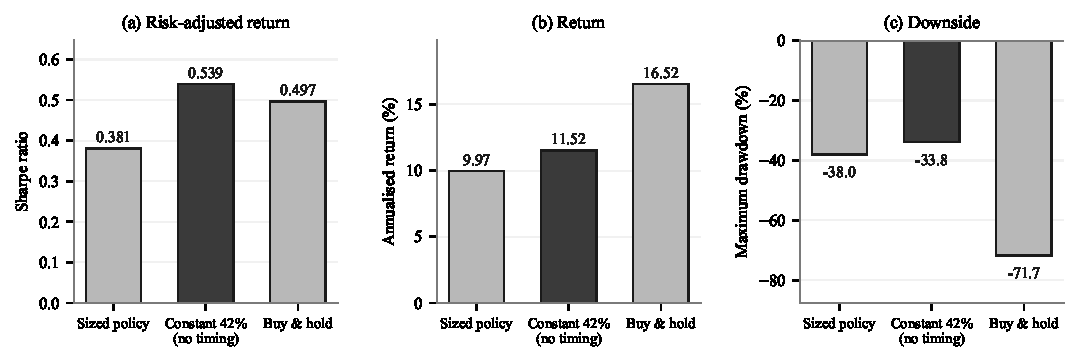
\includegraphics[width=\textwidth]{matched_exposure}
\caption{The matched-exposure control. Holding the sized policy's own average
exposure of 42 percent every day, with no timing whatsoever, beats that policy
on all three measures at once. Buy-and-hold earns the most and falls furthest,
which is why comparing against it alone conceals the failure: reduced exposure
lowers drawdown, so any delevered policy resembles risk management regardless
of what its timing contributes.}\label{fig:exposure}
\end{figure}

The control dominates the sized policy on all three measures simultaneously: a
Sharpe ratio of $0.539$ against $0.381$, an annualised return of $11.52$
percent against $9.97$, and a maximum drawdown of $-33.8$ percent against
$-38.0$. The system's drawdown is $4.2$ percentage points \emph{deeper} than
pure delevering would have delivered, so the timing contributes negatively.

Two internal checks support the reading. The always-invested arm reproduces
buy-and-hold to the digit, confirming the harness. And the first and third arms
attain identical Sharpe ratios ($0.3607$) at exposures of $0.53$ and $0.05$,
a tenfold difference: the Sharpe ratio is invariant to constant rescaling of
exposure, so the three risk profiles of Section~\ref{subsec:riskmgr} are a
leverage dial rather than three distinct strategies.

\subsection{Experiment F: volatility targeting at
scale}\label{subsec:eval-voltarget}

Volatility targeting requires no directional forecast, so it isolates whether
the estimable quantity of Experiment B converts into performance.
Table~\ref{tab:voltarget} tests it across the full universe with turnover costs
charged.

\begin{table}[h]
\caption{Volatility targeting against constant exposure, 196 equities, ten
years, 15 percent annualised volatility target, leverage capped at 3.0, 5 basis
points of turnover cost, idle capital credited at 4 percent.}\label{tab:voltarget}%
\begin{tabular*}{\textwidth}{@{\extracolsep\fill}lrrrr@{}}
\toprule
Arm & Sharpe & Ann.\ return (\%) & Volatility (\%) & Max.\ drawdown (\%) \\
\midrule
Buy and hold                & 0.3371 & 11.17 & 30.18 & $-52.04$ \\
Constant exposure           & 0.3371 &  9.33 & 20.78 & $-38.78$ \\
Volatility targeted         & 0.2746 &  7.79 & 17.96 & $-34.44$ \\
Volatility targeted, lagged & 0.2691 &  7.71 & 18.14 & $-34.94$ \\
\botrule
\end{tabular*}
\footnotetext{Paired $t$-test of volatility targeting against constant
exposure: $t=-8.47$, $p=5.8\times10^{-15}$; targeting wins on 50 of 196 names.}
\end{table}

Volatility targeting is significantly worse than a constant exposure
($t=-8.47$, $p=5.8\times10^{-15}$), prevailing on only 50 of 196 names. It does
reduce drawdown, from $-38.8$ to $-34.4$ percent, and volatility, from $20.8$
to $18.0$ percent, so it delivers what it promises on the risk side while
giving up more return than that risk reduction is worth. Note also that
buy-and-hold and constant exposure record the same Sharpe ratio to four
decimals, which is the invariance property of the previous section reproduced
at universe scale on an independent code path.

This is the sharpest form of the paper's caution. The quantity that Experiment
B shows to be genuinely estimable does not, by itself, produce a better
portfolio.

\subsection{Experiment G: the sealed prospective test}\label{subsec:eval-forward}

Every result above is retrospective, and any pretrained component may have
encountered the period during training. The forward test removes that
possibility by construction. At the time of writing, 240 predictions have been
sealed across five as-of dates at a five-day horizon and 160 have been scored;
no decision was recorded as degraded. Table~\ref{tab:forward} and
Figure~\ref{fig:forward} report the comparison.

\begin{table}[h]
\caption{Sealed prospective test. Arm A invokes the Analyst alone; arm B runs
the full control plane, whose plans dispatched the Researcher, Market, Analyst
and Risk Manager on identical inputs. The paired block restricts to the 40
decisions on which both arms ran.}\label{tab:forward}%
\begin{tabular*}{\textwidth}{@{\extracolsep\fill}lcccc@{}}
\toprule
& Scored & Accuracy [95\% CI] & Median latency & LLM calls/decision \\
\midrule
Arm A, numerical & 120 & 0.4833 \enskip [0.3958, 0.5719] & 1{,}639 ms & 0.00 \\
Arm B, agentic   &  40 & 0.4250 \enskip [0.2851, 0.5781] & 2{,}260 ms & 0.20 \\
\midrule
\multicolumn{5}{@{}l}{\emph{Paired subset, $n=40$}} \\
Arm A & 40 & 0.5250 & \multicolumn{2}{l}{both correct 12, A only 9,} \\
Arm B & 40 & 0.4250 & \multicolumn{2}{l}{B only 5, neither 14} \\
\botrule
\end{tabular*}
\footnotetext{McNemar exact test on the 14 discordant pairs: $p=0.42$. Neither
arm's interval excludes chance.}
\end{table}

\begin{figure}[h]
\centering
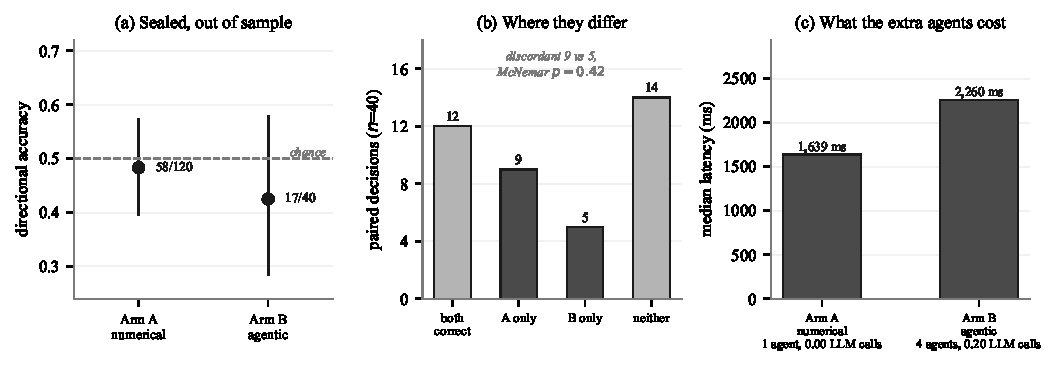
\includegraphics[width=\textwidth]{fig_forward}
\caption{The sealed prospective test. (a) Directional accuracy with 95 percent
Wilson intervals; both arms straddle chance. (b) The paired disagreement, where
the agentic arm wins 5 decisions the numerical arm loses and loses 9 it wins,
a difference the McNemar test cannot separate from noise. (c) What the
additional agents cost per decision.}\label{fig:forward}
\end{figure}

Three readings, all negative or neutral, and all worth stating. Neither arm's
interval excludes chance, so the directional weakness of
Section~\ref{subsec:eval-direction} reproduces prospectively rather than being
an artefact of the retrospective sample. The agentic arm does not beat the
numerical arm; on the paired subset it is nominally worse ($0.425$ against
$0.525$), but with 14 discordant pairs the McNemar test returns $p=0.42$ and
the comparison is uninformative in either direction. And the agentic
configuration costs more, at 1.4 times the median latency plus a small number
of language-model calls.

The abstention result does not yet replicate here either. Sweeping coverage
within each arm produces no monotone trend, but at these sample sizes a
25-percent coverage subset contains 10 to 30 decisions and its Wilson interval
spans roughly $\pm0.17$, so the experiment cannot detect an effect of the size
Table~\ref{tab:abstain} reports. The forward test is currently a check on
direction, not yet a test of selective prediction.

\subsection{Component measurements}\label{subsec:eval-components}

\paragraph{Planner.} On a 33-query evaluation the Planner attains $0.727$
overall (95 percent CI $[0.558, 0.849]$). Splitting by provenance, it reaches
$0.692$ on the 26 queries drawn from a published corpus of retail questions and
$0.857$ on the 7 we authored to exercise the advice and risk-check paths. The
published subset is the fair comparison, and even that is not like-for-like
against the $0.75$ reported for a supervised sentence-encoder classifier
trained on that corpus, since our Planner is zero-shot over an eleven-class
schema it was not fitted to. We report it as a component measurement, not as a
contribution. Per-class recall is perfect on \textsf{advice}, \textsf{assess},
\textsf{data\_point}, \textsf{define} and \textsf{screen}, and zero on
\textsf{summarize}, whose three queries are absorbed into
\textsf{company\_profile} and \textsf{risk\_check}. With $n=33$ the interval is
wide enough that only the coarsest conclusion is supported: routing works well
enough to make dynamic dispatch meaningful, and \textsf{summarize} needs
disambiguation. A larger annotated set is the obvious next step.

\paragraph{Researcher.} Not scored retrospectively, for the reason given in
Section~\ref{subsec:researcher}. In the prospective arm it returned evidence
without a degraded flag on all 40 agentic decisions.

\paragraph{Robustness at universe scale.} A three-name, ten-year replication of
the full sized policy returns a mean Sharpe ratio of $0.279$ against $0.611$
for buy-and-hold, winning on none of the three. We report it as a consistency
check on the direction of the effect rather than as evidence about the
population, since three correlated large-capitalisation names carry almost no
independent information.

%% ==================================================================
\section{How much data would settle this?}\label{sec:power}
%% ==================================================================

Every performance comparison above is bounded by a constraint that is rarely
stated in this literature, and which we believe deserves to be a result in its
own right.

Calibrating to the holdout gives a strategy-to-benchmark correlation of $0.552$
and a benchmark Sharpe ratio of $+0.314$. Applying the variance expression of
\citet{jobson1981performance} with the correction of
\citet{memmel2003performance} yields Table~\ref{tab:power} and
Figure~\ref{fig:power}.

\begin{table}[h]
\caption{Trading days required to detect a true difference in Sharpe ratio at
80 percent power and a 5 percent false-positive rate, against a benchmark
correlated $0.55$ with the strategy.}\label{tab:power}%
\begin{tabular*}{\textwidth}{@{\extracolsep\fill}rrrr@{}}
\toprule
True Sharpe difference & Required days & Years & Power at our 398-day holdout \\
\midrule
$+0.30$ & 19{,}692 & 78.1 & 5.9\% \\
$+0.50$ &  7{,}093 & 28.1 & 9.7\% \\
$+1.00$ &  1{,}778 &  7.1 & 26.3\% \\
\botrule
\end{tabular*}
\end{table}

\begin{figure}[h]
\centering
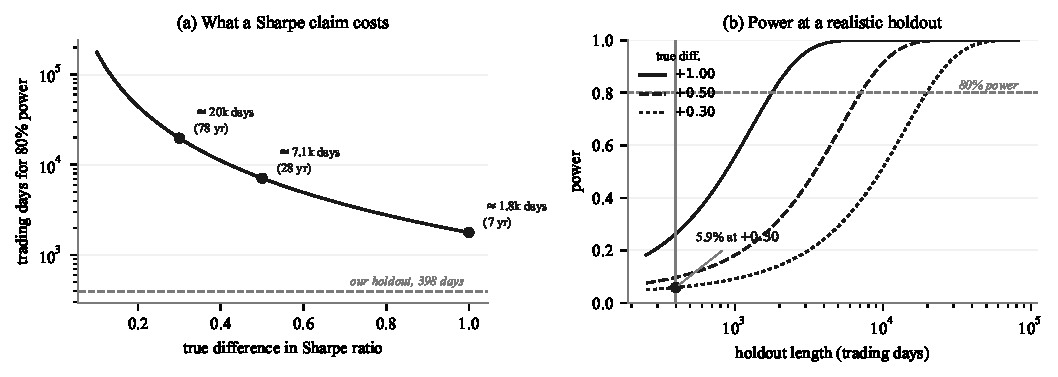
\includegraphics[width=\textwidth]{fig_power}
\caption{What a risk-adjusted-return claim costs in data. (a) Trading days
required for 80 percent power, against the size of the true Sharpe difference;
the dashed line is our own holdout. (b) Power against holdout length for three
effect sizes; at 398 days the test has 5.9 percent power against a $+0.30$
difference, barely above the 5 percent false-positive
rate.}\label{fig:power}
\end{figure}

A true Sharpe improvement of $+0.30$, a large and economically meaningful
effect, requires roughly 19,700 trading days, or 78 years, per name. Our
holdout is 398 days and its power against that effect is $5.9$ percent. The
experiment could not have succeeded whatever the strategy did.

Breadth does not rescue it, because contemporaneous equity returns are
correlated. At a cross-sectional correlation of $0.35$, five hundred names
supply roughly $2.85$ effective independent units against $2.08$ for five: two
orders of magnitude more data buy less than a $40$ percent increase in
effective sample size. This is why we do not present the 196-name universe as
evidence that the system works, and why our own headline results are accuracy
and calibration rather than Sharpe superiority. Directional accuracy and
calibration converge within hundreds of observations; Sharpe differences do not.

The accompanying tests behave exactly as this arithmetic predicts. The pooled
Sharpe difference against buy-and-hold is $-0.162$ with a 95 percent interval
of $[-0.752, +0.428]$ and $p=0.599$; no individual name produces an interval
excluding zero; the superior-predictive-ability test of \citet{hansen2005spa},
applied over the risk-profile choice, returns $p=1.0000$; and six pairwise
component comparisons, including the system against a textbook moving-average
crossover and against time-series momentum
\citep{moskowitz2012timeseries}, yield no significant difference.

The correct reading is not that the agents fail. It is that this experiment
cannot distinguish them from a moving average or from doing nothing, and
neither can any published experiment of comparable size. We state this as a
claim about \emph{decidability}, not about the truth of others' results: a
reported win at these sample sizes is not false, it is unfalsifiable.

%% ==================================================================
\section{Discussion}\label{sec:discussion}
%% ==================================================================

\subsection{Finding 1: raw directional prediction is weak}\label{subsec:disc-direction}

Across 196 equities and a decade, directional forecasting from technical
information is not merely weak but adverse at short horizons, and the finding
reproduces in a sealed prospective sample where contamination is impossible.
This is consistent with weak-form efficiency \citep{fama1970efficient} and with
the failure of comparable systems to outperform passive exposure over long
spans \citep{li2025finsaber}. The implication is not that the models are poorly
tuned; it is that the target is wrong. A literature that tunes harder against
this target is optimising a quantity its own data show to be unavailable.

\subsection{Finding 2: uncertainty carries more
information}\label{subsec:disc-uncertainty}

Volatility and drawdown are substantially more estimable from identical inputs,
by a factor of roughly seven in rank correlation. The asymmetry is actionable
rather than merely descriptive: an Analyst emitting a distribution supports
position sizing, downside constraints and abstention, none of which require
knowing which way a price will move.

Two qualifications keep the claim honest. Volatility predictability is not
profitability: Section~\ref{subsec:eval-voltarget} shows a well-estimated
$\hat{\sigma}$ producing a \emph{worse} portfolio when used to scale exposure,
so a dependable dispersion estimate improves risk control without generating
return. And the derived risk quantities are not yet calibrated well enough to
carry weight, being biased low by $11$ percent and sloping the wrong way across
the reliability curve. Estimability is a precondition for usefulness, not a
substitute for it.

Our volatility-targeting result appears to sit against
\citet{moreira2017volatility}, who report gains from volatility management. We
suspect the difference is one of aggregation, since their result concerns the
market portfolio while ours concerns single names, where idiosyncratic variance
dominates and the signal is correspondingly noisier. We have not tested this
explanation and flag it as unresolved.

\subsection{Finding 3: selective prediction is the mechanism that
survives}\label{subsec:disc-abstention}

Confidence-based abstention raises accuracy monotonically as coverage narrows,
with every interval excluding chance, even though the underlying point forecast
is anti-predictive. An agent that forecasts poorly can still know when to
decline, and that ordering is exploitable in a way the point estimate is not.

For an agentic system specifically, this reframes what the intermediate agents
are for. Their value is not that they vote more accurately but that they emit
quantities whose reliability can be ranked and audited. Abstention is the
interface through which that ranking reaches the user.

\subsection{Finding 4: exposure must be controlled before skill can be
claimed}\label{subsec:disc-eval}

An evaluation comparing only against buy-and-hold cannot detect the sizing
failure of Section~\ref{subsec:eval-sizing}, because reduced exposure lowers
drawdown and thereby presents as risk management. A matched-exposure control
should accompany any such comparison; it costs nothing to compute and it
reversed the sign of our own conclusion.

The same reasoning applies to execution timing. Applying a decision to the
session whose close produced it inflated the mean Sharpe ratio from $0.192$ to
$0.724$ in an earlier revision of this system and flipped the headline from two
of five names to four. The defect presented as skill precisely because the
comparison baseline was correctly lagged, so the contamination appeared only in
the treatment arm and every diagnostic looked healthy. Nine regression tests now
assert temporal alignment directly. That episode is the empirical counterpart
to the property \citet{fonseca2026lookahead} formalise, and the kind of case
\citet{benhenda2026lookaheadbench} invite benchmark contributors to supply.

\subsection{What the decomposition does and does not
buy}\label{subsec:disc-agents}

The decomposition's demonstrated benefit here is epistemic rather than
predictive. Because the Planner, Analyst and Risk Manager are separable and
each emits a typed, timestamped, confidence-bearing message, the system's
failure could be localised to the Analyst's choice of target rather than
attributed vaguely to the architecture. That is the answer to RQ1, and it is
what made every other result in this paper reachable.

What the decomposition did \emph{not} buy is accuracy. In the one experiment
that compares configurations directly and without contamination, the fully
agentic arm was statistically indistinguishable from the single-agent arm while
costing more (Section~\ref{subsec:eval-forward}). We therefore make the weaker claim,
because it is the one our measurements support: agentic organisation is
justified here by auditability and by the per-agent evaluation it enables, not
by a demonstrated improvement in decision quality. Establishing the stronger
claim would require the coordination and cost metrics that
\citet{nguyen2026reliable} propose, over a far larger prospective sample.

%% ==================================================================
\section{Limitations and future work}\label{sec:limitations}
%% ==================================================================

The universe was selected at the end of the sample, so survivorship flatters
every retrospective column; \citet{li2025finsaber} handle this properly and we
do not. No historical news or fundamental archive was available at our access
tier, so the Researcher contributes nothing to the retrospective results and is
evaluated only prospectively. The prospective test itself is small, at 160
scored decisions across five as-of dates and a single five-day horizon, which
is why it can reject nothing. The Planner is measured on 33 queries, an
interval too wide to support a comparison against published classifiers. The
derived downside probabilities are miscalibrated in a structured way and should
not yet be relied on. The volatility-targeting result is unreconciled with
\citet{moreira2017volatility}. Retrospective results assume execution at
closing prices with turnover costs charged in one experiment and not the other,
as Section~\ref{subsec:protocol-costs} sets out. Finally, the control plane
depends on a language model for planning, which introduces an external service
dependency, a cost, and a source of run-to-run variation that we mitigate with
schema validation and caching but do not eliminate.

Four extensions follow directly. Range-based volatility estimators should
improve $\hat{\sigma}$ and, through Equation~\eqref{eq:dd}, every derived
quantity that inherits its bias. An archival news corpus would let the
Researcher enter retrospective evaluation. The prospective test should be
extended in breadth and duration until it can test selective prediction rather
than only direction. And the abstention threshold, currently a fixed rule,
should be set by the risk--coverage curve the deployment actually faces.

%% ==================================================================
\section{Conclusion}\label{sec:conclusion}
%% ==================================================================

We asked what a financial agent should predict. Measured across 196 equities
and ten years, the direction of price movement is anti-predictive at short
horizons and no better than chance at longer ones, while realised volatility
and forward drawdown are estimated roughly seven times better from identical
inputs. Confidence-aware abstention raises directional accuracy from $52.1$ to
$57.5$ percent as coverage narrows, every interval excluding chance, and is the
one mechanism in the system that survives scrutiny. A matched-exposure control
shows that the sizing policy's apparent risk management is reduced exposure
rather than timing skill, and a power analysis shows that the risk-adjusted
comparisons this literature relies on are undecidable at the sample sizes it
uses.

The recommendation follows from the measurement rather than from the
architecture. Systems and evaluations built on directional forecasting should
be rebuilt on uncertainty estimation and selective prediction, and any
risk-management claim should be reported beside an exposure-matched control.
The agentic decomposition earns its place here not because it predicts better,
which we could not demonstrate, but because it is what allowed the failure to
be located at all.

%% ==================================================================
\backmatter

%%==================================================================%%
%% Digital Finance requires a "Statements and Declarations" section.
%% Complete every TODO below before submission.
%%==================================================================%%

\section*{Statements and Declarations}

\bmhead{Funding}
%% TODO: state funding sources, or keep the sentence below if none.
The authors declare that no funds, grants or other support were received during
the preparation of this manuscript.

\bmhead{Competing interests}
The authors have no competing interests to declare that are relevant to the
content of this article.

\bmhead{Ethics approval}
Not applicable. This study did not involve human participants or animals.

\bmhead{Data availability}
%% TODO: add the public repository or archive URL before submission.
All price data used in this study are daily open, high, low, close and volume
series for publicly listed United States equities obtained from a public
market-data provider. The evaluation code, the sealed prospective prediction
log, the derived result files reproducing every table and figure, and the
parameter settings required to regenerate them are available from the
corresponding author on reasonable request and are being prepared for public
release.

\bmhead{Author contributions}
%% TODO: confirm with all authors before submission.
Mansi designed and implemented the system, designed and ran the evaluation, and
wrote the manuscript. Sudesh Rani and Kanu Goel supervised the work, advised on
the evaluation design, and reviewed and edited the manuscript. All authors read
and approved the final manuscript.

%%==================================================================%%

\bibliography{references}

\end{document}
